\documentclass[a4paper,10pt]{article}
\usepackage[utf8]{inputenc}
\usepackage{graphicx}

%opening
\title{}
\author{Bram van Es}

\begin{document}

\maketitle

\begin{abstract}
Short description of results/methods
\end{abstract}

\section{General approach}
%
We have the following dataset:
\begin{itemize}
 \item ECG: $646$ columns with aggregated data from ElectroCardioGram's, 
 \item CELLDYN: $40$ columns
 \item Phenotypical: age, gender, BMI
 \item Clinical: historical clinically relevant information (hypertension, hyperchol, diabetes, etc.)
 \item heartscore: ..
 \item troponine: both the initial measurement and the slope obtained after a second measurement
\end{itemize}

We first handled the NaN's in the dataset; we have 5 columns with NaN's for 8\% of the samples, 4 of them have a specific clinical meaning, the other is BMI. The 4 clinical features are related to the P-R interval of the ECG 
and the absence of these specific features can signal atrium fibrillation. For this reason we map
all non-NaN's in these columns to $1$ and all NaN's to $0$. For the BMI we simply take the median given it's low variance in the dataset, and given the fact that we are more interested in the impact of adding CELLDYN data. 

We expanded the CELLDYN dataset using pairwise feature combinations, specifically we applied
$A/(A+B+\epsilon)$ and $\sqrt{A\cdot B}$, where $A$ and $B$ are different celldyn features.

We considered several transformations (quantile/minmax/standard) but the non-transformed features seemed to perform
the best. We also considered removing the collinearity but it did not positively affect the predictive accuracy
of the models. We prune the data by including only minimally informative features, which was based on multiple statistic distance metrics such as Anova, Kolmogorov-Smirnov, the 1st and 2nd Wasserstein distance.
%

We define the following feature sets:
\begin{enumerate}
 \item age, gender, BMI, ECG, (CELLDYN)
 \item age, gender, BMI, ECG, initial troponine, (CELLDYN)
 \item age, gender, BMI, ECG, initial troponine, history, (CELLDYN)
 \item age, gender, BMI, ECG, initial troponine, history, heartscore, (CELLDYN)
 \item age, gender, BMI, ECG, initial troponine, history, heartscore, troponine slope, (CELLDYN)
\end{enumerate}
% 
where for each feature set we have a with/without CELLDYN variant. 

For each of these feature set we apply 10-fold cross-validation on an ensemble of machine learning models using a calibrated voting classifier. The models used are: XGboost, LightGBM, ExtraTrees, RandomForest and $\mu$-SVM. 
For comparison we use a second ensemble of a convolutional network and a fully connected neural network.
For the application of the neural network we did apply dimension reduction and feature transformation, namely 
$PCA$ and a quantile transformation.


%The third model is a dummy model, a logistic regressor using only age, gender and BMI.
%The fourth model is a reference model, a logistic regressor using only age, gender, BMI, heart %score and troponine information (initial plus the slope).

%
\section{Results}
%
The classes are slightly imbalanced; the NSTEMI's are underrepresented with $30\%$, in the modelling we compensate for this using higher target weights for the NSTEMI's. 

\subsection{Exploration}
%
\begin{center}
 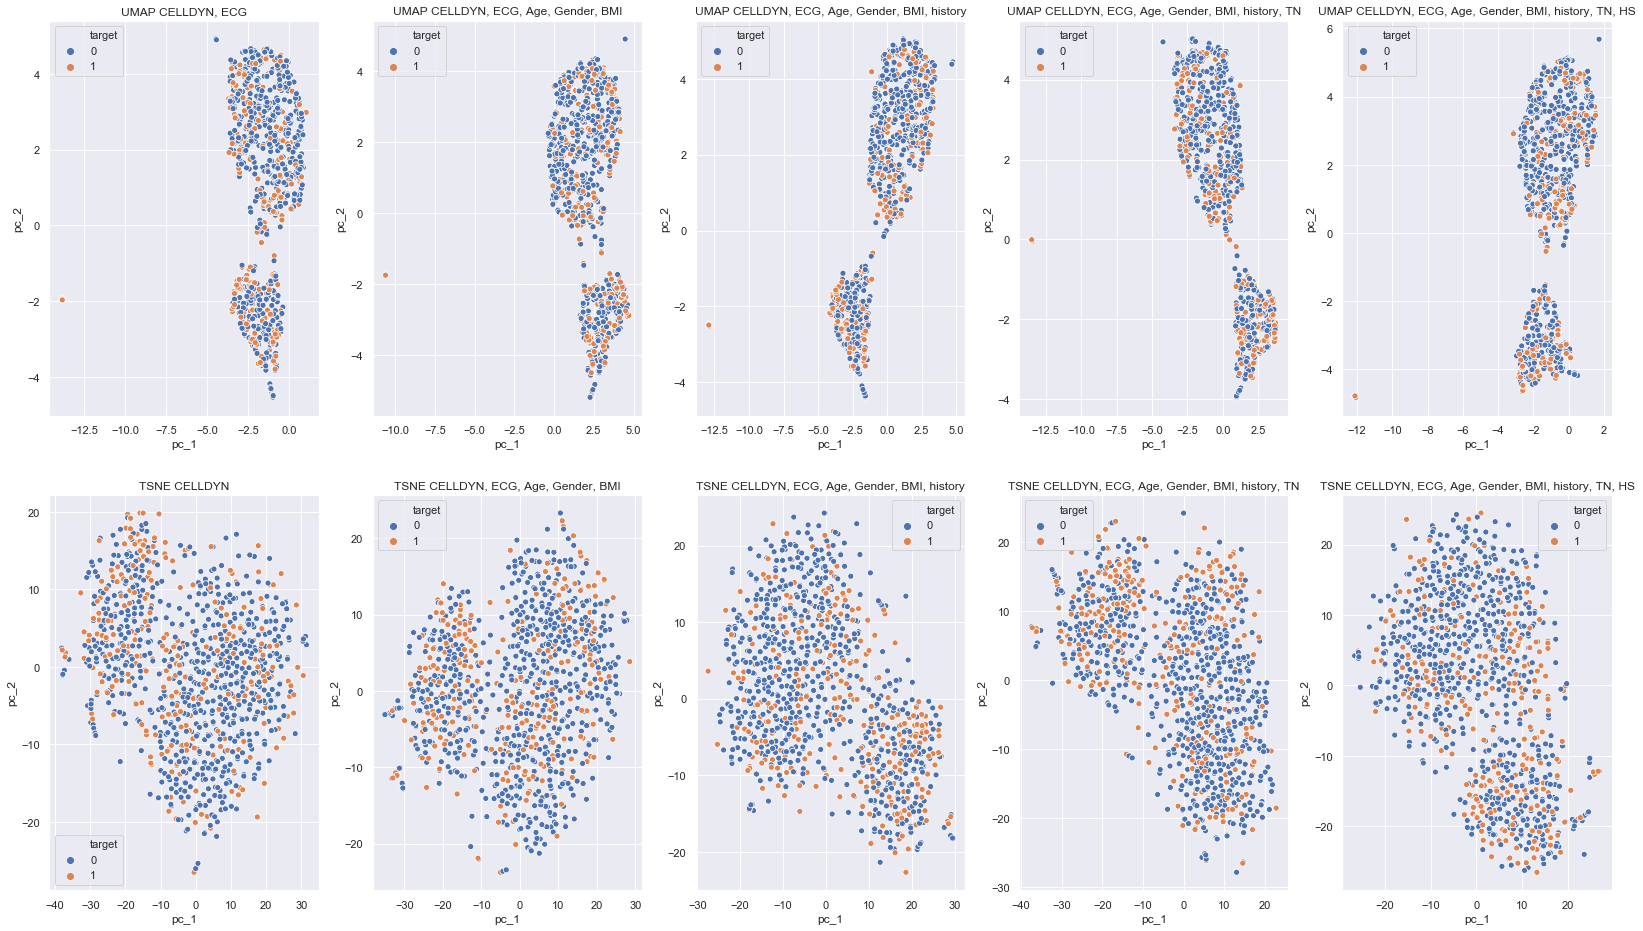
\includegraphics[bb=0 0 1643 931,scale=0.25,keepaspectratio=true]{images/Clustering.png}
 % Clustering.png: 1643x931 px, 72dpi, 57.97x32.85 cm, bb=0 0 1643 931
\end{center}
%
Using unsupervised clustering on UMAP and t-SNE reduced data we see that using CELLDYN data we can split the patients into two clusters, these two clusters persist when we add more data. 
%
Using LDA we look at the linear separability of the NSTEMI/non-NSTEMI patients.
%
\begin{center}
 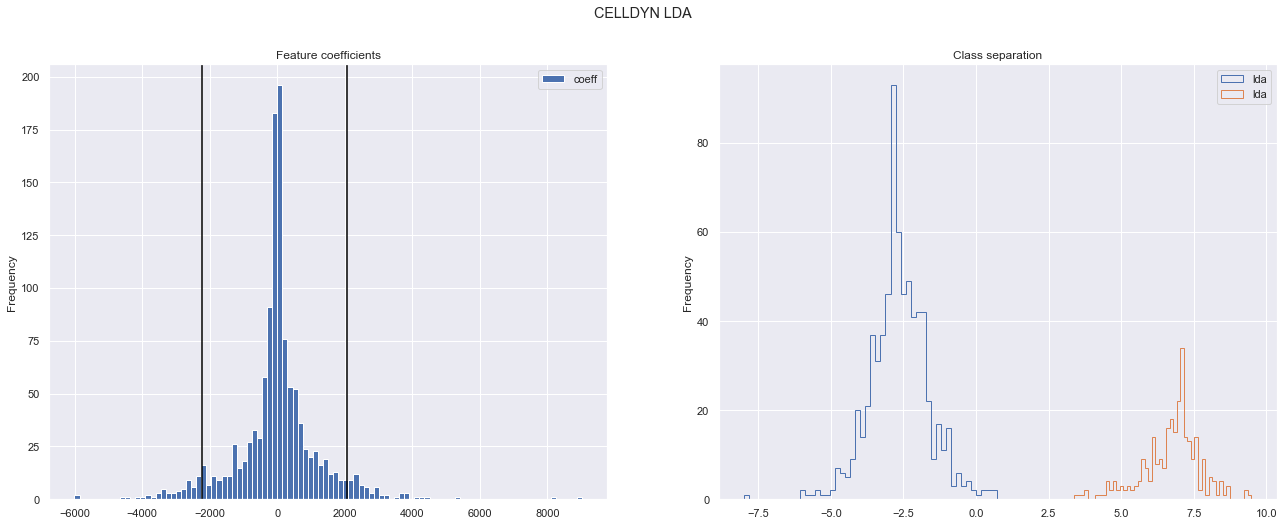
\includegraphics[bb=0 0 1284 526,scale=0.2]{images/LDA_full.png}
 % LDA_full.png: 1284x526 px, 72dpi, 45.31x18.56 cm, bb=0 0 1284 526
\end{center}
%
The LDA transform suggests that the two classes are linearly separable. To test this we generate
an LDA model on a training set and apply it to a test set, which results in poor performance, with the AUC 
close to $0.50$. This suggests that a combination of the following is at play  
\begin{itemize}
\item the target NSTEMI/non-NSTEMI can only be separated using non-linear methods
\item high sensitivity of class separation to outliers (should be taken care of with quantile transformations)
\item high variance of variance within dataset; i.e. there are a lot of patient segmentations
\end{itemize}
%
We repeated the LDA using quantile transformed variable and we found a similar result, and the same 
when we applied synthetic upsampling using SMOTE.
%
Using feature set 3 we test the following classifiers; LDA, LR, RF, $\mu$-SVM, $3$ layered MLP, XGB and LGBM, and an ensemble of RF, $\mu$-SVM, LR and MLP. 
%
\begin{center}
 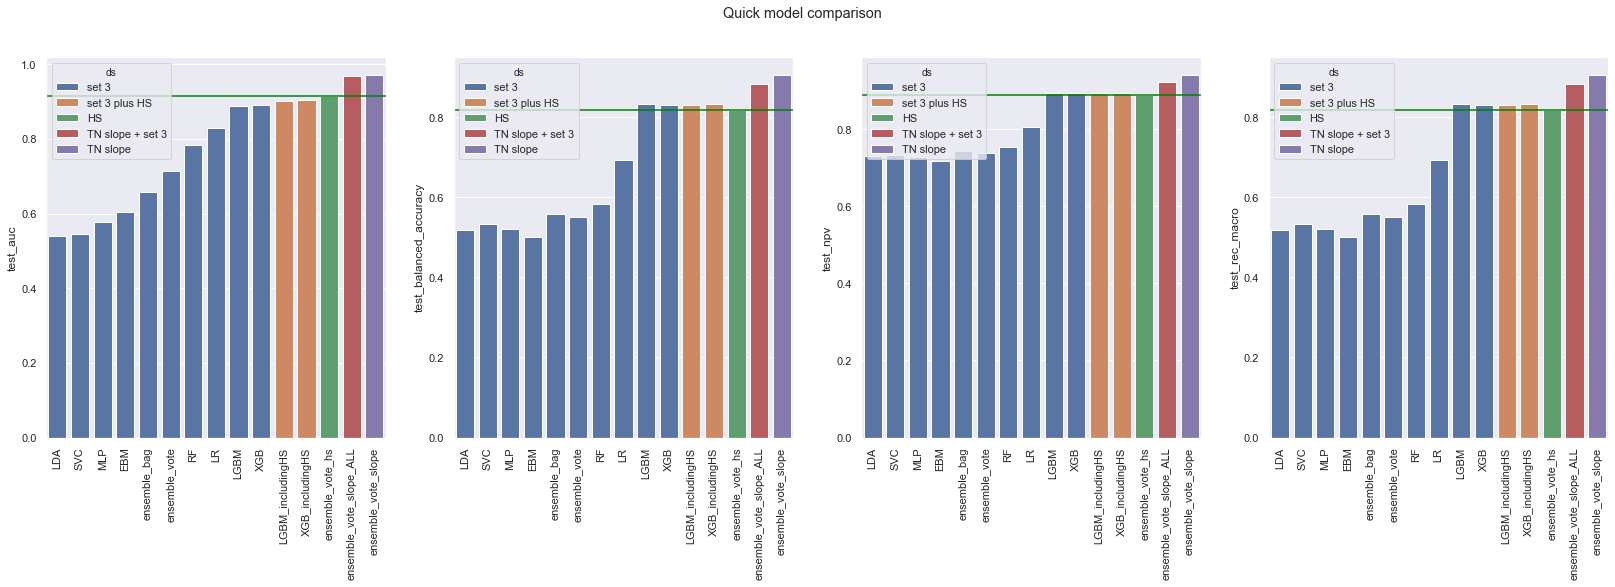
\includegraphics[bb=0 0 1615 587,scale=0.2,keepaspectratio=true]{images/perf_bar.png}
 % perf_bar.png: 1615x587 px, 72dpi, 56.99x20.71 cm, bb=0 0 1615 587
\end{center}

In terms of AUC/F1/precision and NPV the XGB and LGBM models on featureset 3 are an improvement over heartscore or on par. When we combine the troponine data (including the slope) with the other available data we do not see an improvement over just the troponine data. 
%
\begin{center}
 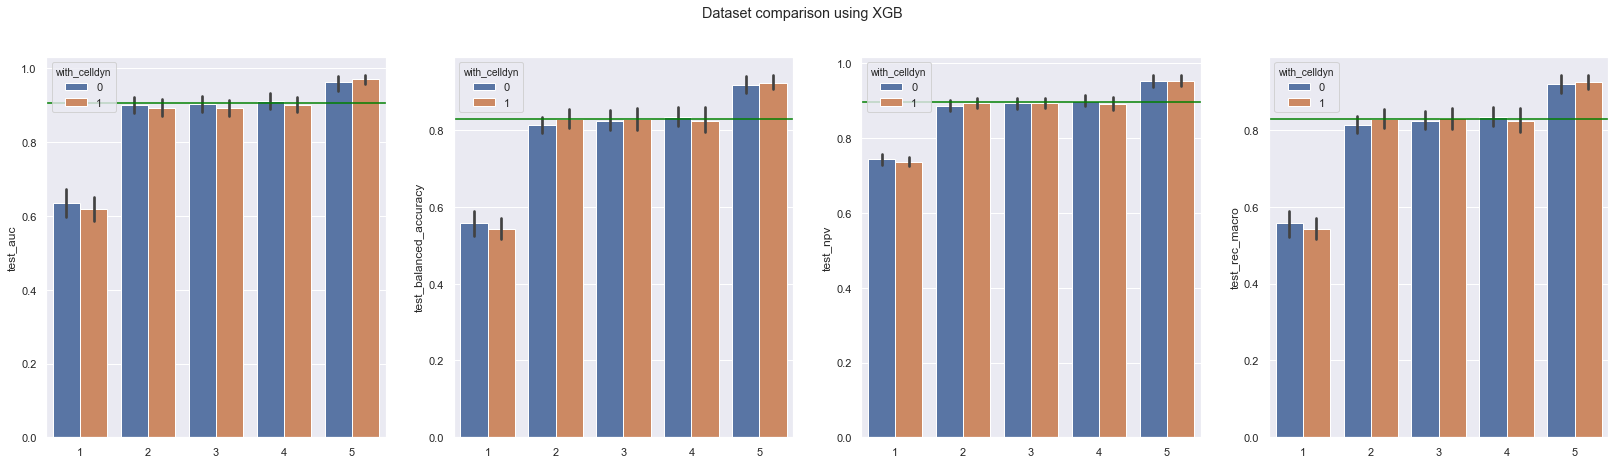
\includegraphics[bb=0 0 1615 464,scale=0.2,keepaspectratio=true]{images/perf_bar_ds.png}
 % perf_bar_ds.png: 1615x464 px, 72dpi, 56.99x16.37 cm, bb=0 0 1615 464
\end{center}
%
The scores for feature sets 2,3,4 are comparable, the results with and without CELLDYN 
are not significantly different.

%
In terms of feature importances: the top-100 features is populated by 
%
%
\subsection{Cross validation}
%
Continuing with the model testing we run a 10-fold cross-validation with an ensemble of XGB, LGBM, RF, ET and $\mu$-SVM.
%%
\begin{center}
 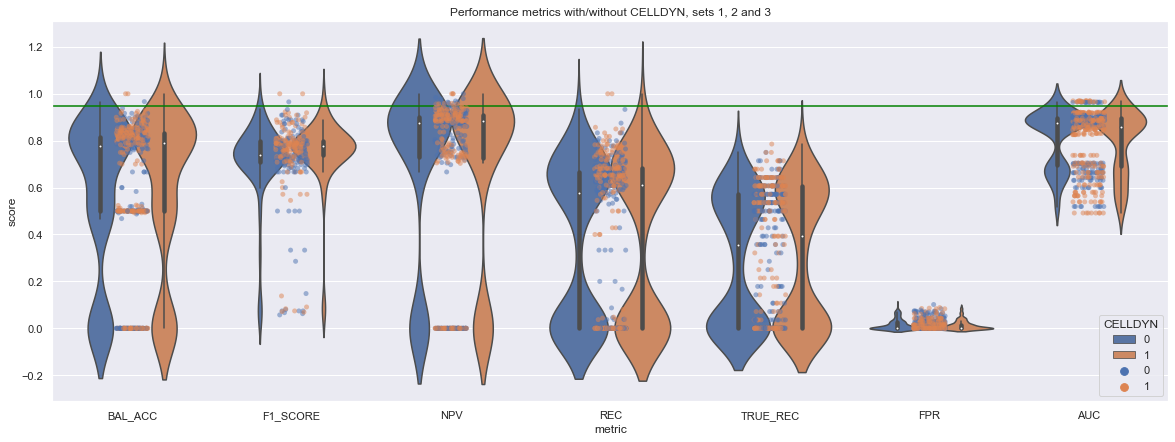
\includegraphics[bb=0 0 1175 442,scale=0.3]{images/violin_ensemble_1.png}
 % violin_ensemble_1.png: 1175x442 px, 72dpi, 41.46x15.60 cm, bb=0 0 1175 442
\end{center}
%
For the first model ensemble we see a slight improvement in NPV/F1 scores when we add CELLDYN to the feature sets, however this is not significant according to the Kolmogorov-Smirnov test ($p=0.1$), and for the second model ensemble we see a slight deterioration (with $p<0.01$).
%
Independently we see that a featureset with age, gender, BMI and CELLDYN has some predictive value.
\begin{center}
 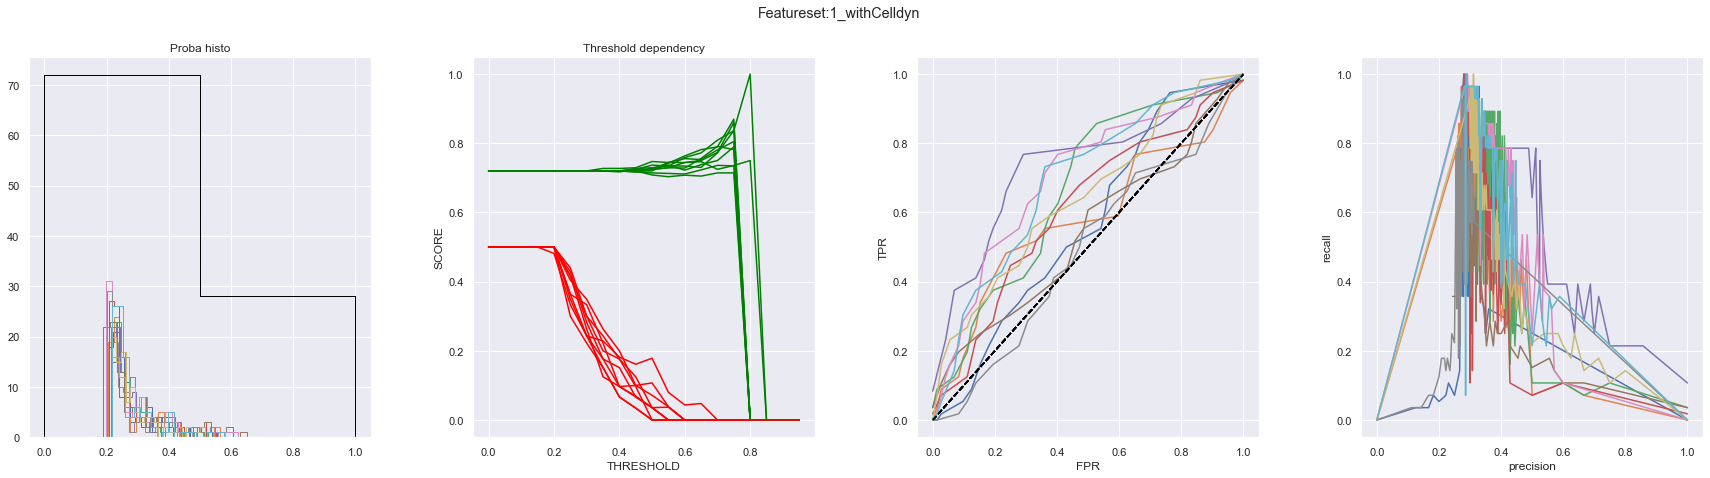
\includegraphics[bb=0 0 1710 478,scale=0.2,keepaspectratio=true]{images/metric_plots_set1_ensemble_1.png}
 % metric_plots_set1_ensemble_1.png: 1710x478 px, 72dpi, 60.34x16.87 cm, bb=0 0 1710 478
\end{center}
%
Adding troponine significantly improves the result and brings the accuracy on par with feature sets 3 and 4 that include the tailor made heart score and the historical clinical information.

\begin{center}
 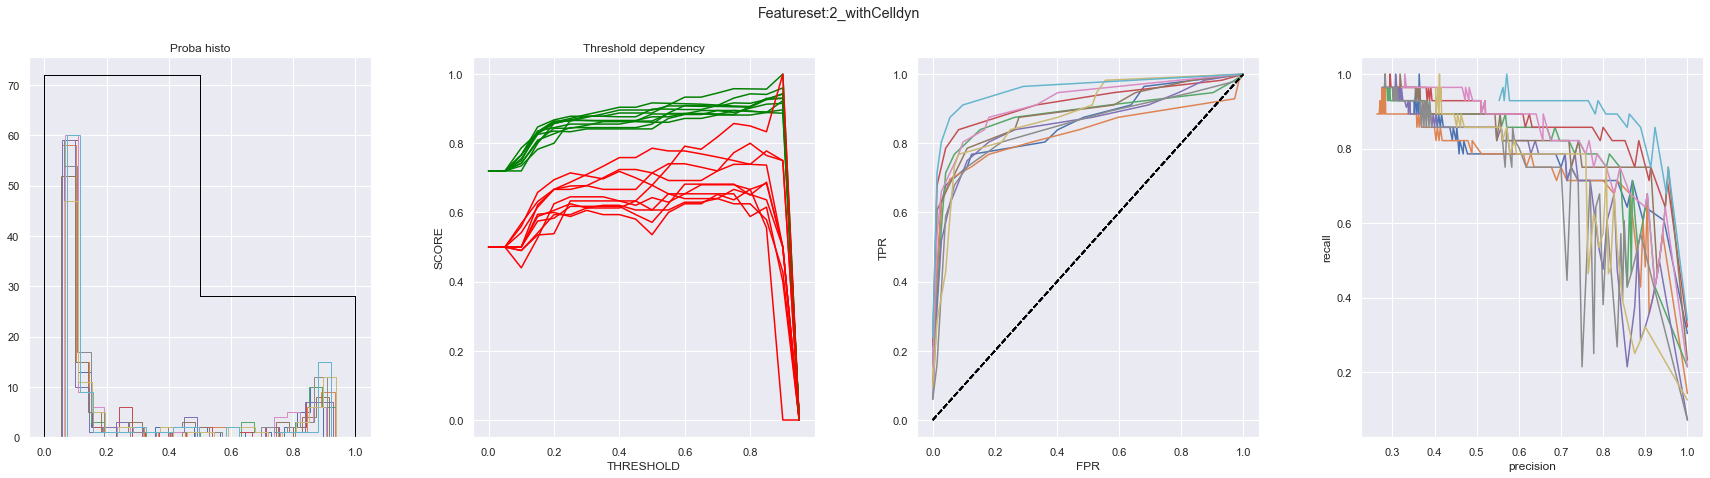
\includegraphics[bb=0 0 1710 478,scale=0.2,keepaspectratio=true]{images/metric_plots_set2_ensemble_1.png}
 % metric_plots_set2_ensemble_1.png: 1710x478 px, 72dpi, 60.34x16.87 cm, bb=0 0 1710 478
\end{center}
%
%
\begin{center}
 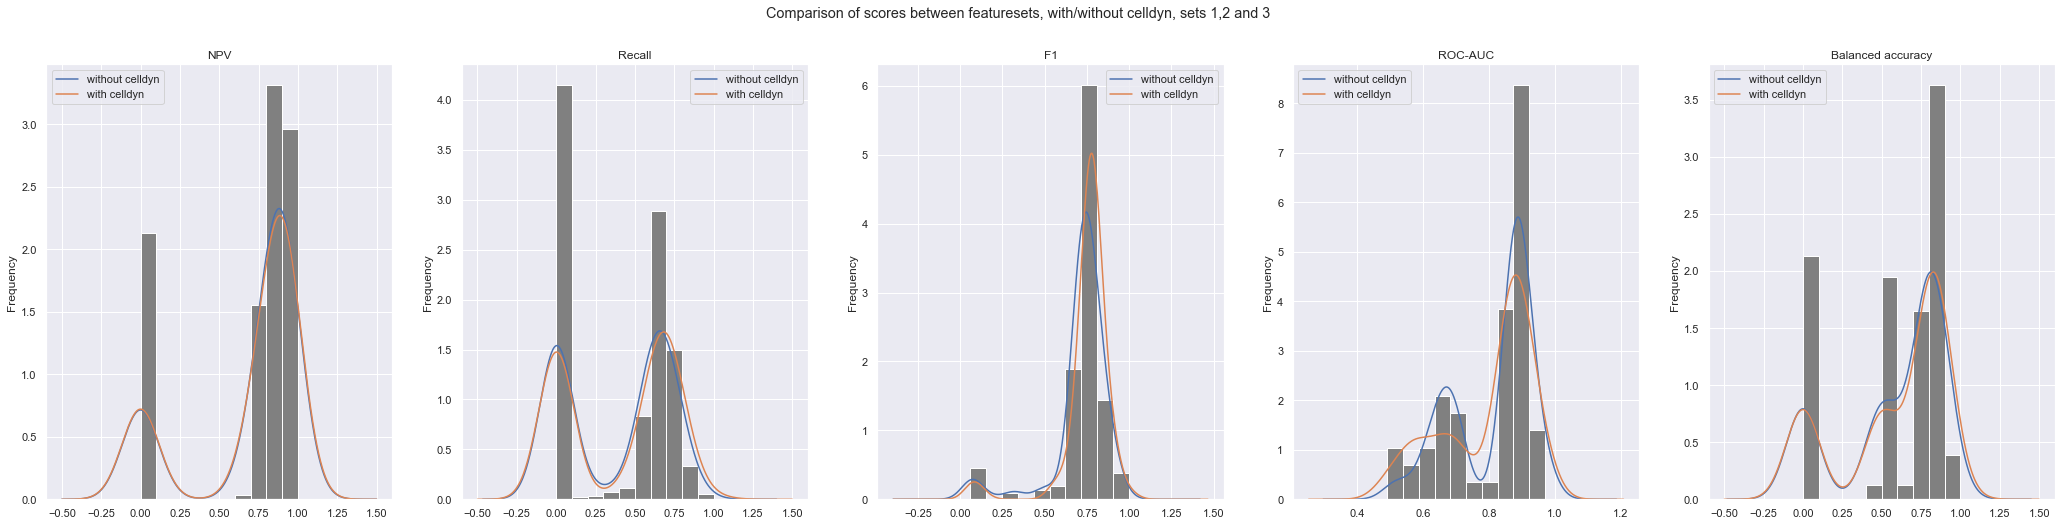
\includegraphics[bb=0 0 2062 526,scale=0.2,keepaspectratio=true]{images/metric_distro_ensemble_1.png}
 % metric_distro_ensemble_1.png: 2062x526 px, 72dpi, 72.76x18.56 cm, bb=0 0 2062 526
\end{center}

%
We also see that for both model ensembles there are one or two folds in the CV that produce a 
trivial model with all zeros, supporting the idea that the variance within the population is very large, 
leading to non-informative patient selections. To overcome this we might benefit from oversampling the minority class and by tweaking the target weights.

%
We conclude that 
\begin{itemize}
\item separating NSTEMI from non-NSTEMI patients is a highly non-linear problem 
\item CELLDYN clusters the heart patients in two distinct groups, however they are not predictive for the target
\item CELLDYN can improve the ability to detect NSTEMI's but is not sufficiently accurate as a standalone predictor (with the used set of CELLDYN features) 
\item using readily available data at patient-intake an accurate prediction can be made regarding NSTEMI's
\end{itemize}

\section{Suggestions}
There are things we can do to improve the results;
%
\begin{itemize}
\item look for specific patients groups for which CELLDYN can provide significantly improved predictive accuracy, for this we need more data
\item add more CELLDYN features
\item parameter optimisation of the models, including the target weights to improve the NPV
\item inter-dataset feature enrichment 
\item remove outlying samples
\item rigorously prune the ECG/CELLDYN data t
\item apply synthetic over-sampling 
\item mine clinical reports for more sample features
\item different thresholds NSTEMI and non-NSTEMI's predictions
\item apply AutoML libraries such as AutoGluon, AutoKeras and TPOT
\end{itemize}

\end{document}
